\documentclass[11pt,a4paper]{article}
\usepackage[margin=2.3cm]{geometry}
\IfFileExists{lmodern.sty}{\usepackage{lmodern}}{}
\usepackage[T1]{fontenc}
\usepackage{titlesec,tabularx,longtable,booktabs,array,enumitem,xcolor,fancyhdr,amsmath}
\usepackage{listings}
\usepackage{tikz}
\usetikzlibrary{arrows.meta,positioning,fit,calc,shapes.geometric,backgrounds}
\usepackage[hyphens]{url}
\usepackage{hyperref}

\definecolor{headcolor}{RGB}{15,70,60}
\definecolor{boxa}{RGB}{226,239,236}
\definecolor{boxb}{RGB}{238,242,250}
\definecolor{boxc}{RGB}{250,243,230}
\definecolor{boxd}{RGB}{245,245,245}
\definecolor{edge}{RGB}{70,70,70}
\hypersetup{colorlinks=true,linkcolor=headcolor,urlcolor=headcolor,
  pdftitle={TrustBazaar System Design - Unit 8: Frontend},
  pdfauthor={S. M. Nihal Ahmed, Afrim Hossen Khan, Sabikun Nahar Sinthia}}

\titleformat{\section}{\normalfont\Large\bfseries\color{headcolor}}{\thesection}{10pt}{}
\titleformat{\subsection}{\normalfont\large\bfseries}{\thesubsection}{8pt}{}
\titleformat{\subsubsection}{\normalfont\normalsize\bfseries}{\thesubsubsection}{6pt}{}
\pagestyle{fancy}\fancyhf{}
\fancyhead[L]{System Design Document}\fancyhead[R]{Unit 8: Frontend}
\fancyfoot[C]{\thepage}\renewcommand{\headrulewidth}{0.4pt}\setlength{\headheight}{14pt}
\setlength{\emergencystretch}{3em}
\setlength{\parskip}{0.45em}\setlength{\parindent}{0pt}

\lstdefinelanguage{SQLpg}{morekeywords={CREATE,TABLE,TYPE,AS,ENUM,PRIMARY,KEY,REFERENCES,NOT,NULL,DEFAULT,CHECK,UNIQUE,INDEX,ON,WHERE,TRIGGER,BEFORE,INSERT,UPDATE,DELETE,FOR,EACH,ROW,EXECUTE,FUNCTION,RETURNS,LANGUAGE,BEGIN,END,IF,THEN,ELSE,RETURN,SELECT,FROM,INTO,ORDER,BY,DESC,LIMIT,GRANT,REVOKE,TO,SCHEMA,EXTENSION,EXISTS,OR,AND,IN,IS,ALTER,ADD,FOREIGN,GENERATED,ALWAYS,IDENTITY,DEFERRABLE,INITIALLY,DEFERRED,DECLARE,PERFORM,LOOP,RAISE,EXCEPTION,USING,DISTINCT,ROLE,LOGIN,USAGE,ALL,TABLES,STABLE,DO},sensitive=false,morecomment=[l]{--},morestring=[b]'}
\lstdefinelanguage{JS}{morekeywords={import,export,from,const,let,async,await,function,return,new,if,throw,try,catch,for,of,true,false,null},sensitive=true,morecomment=[l]{//},morestring=[b]",morestring=[b]`}
\lstset{basicstyle=\ttfamily\scriptsize,columns=fullflexible,keepspaces=true,breaklines=true,
  keywordstyle=\color{headcolor}\bfseries,commentstyle=\color{gray}\itshape,frame=single,rulecolor=\color{gray!40},
  upquote=true,literate={–}{{--}}1}

\newenvironment{dtable}[1]{\small\begin{longtable}{#1}}{\end{longtable}}

\begin{document}
\begin{titlepage}
\centering
\vspace*{1cm}
{\Large Daffodil International University}\\[0.2cm]
{\large Department of Software Engineering}\\[2cm]
\rule{\linewidth}{0.5pt}\\[0.4cm]
{\huge\bfseries System Design Document}\\[0.3cm]
{\LARGE Unit 8: Frontend}\\[0.3cm]
{\large TrustBazaar: A Verified Peer-to-Peer Auction and Marketplace Platform for Used Goods}\\[0.2cm]
\rule{\linewidth}{0.5pt}\\[1.6cm]
{\large S. M. Nihal Ahmed (232-35-002)\\[0.1cm] Afrim Hossen Khan (232-35-076)\\[0.1cm] Sabikun Nahar Sinthia (232-35-475)}\\[1.6cm]
\begin{tabular}{|l|>{\raggedright\arraybackslash}p{8cm}|}
\hline
\textbf{Status} & Draft for team review \\ \hline
\textbf{Version} & 0.1, 18 October 2026 \\ \hline
\textbf{Implements} & SRS v2.0 (\texttt{docs/srs.tex}) \\ \hline
\textbf{Depends on} & Units 1 to 7 (their HTTP APIs, live events and rules) \\ \hline
\textbf{Reference code} & \texttt{docs/design/web/}, tested in Node, Chromium and nginx (83 checks, Appendix B) \\ \hline
\end{tabular}
\vfill
\end{titlepage}
\tableofcontents
\newpage
\section{Introduction}

\subsection{Purpose}
This document is the eighth unit of TrustBazaar's System Design Document: the web client. Units~1 to~7 designed the backend, each with its HTTP API, its live events and the rules the client must follow. This unit decides how one React application turns them into the screens of the SRS (IF-UI-01 to IF-UI-10). It covers:
\begin{itemize}[nosep]
  \item the structure of the application: four HTML documents (the user app, the staff console, the KYC capture page and the credential pages), routing, and the folders per unit;
  \item how the client talks to the backend: one API client that follows Unit~1's cookie, CSRF, refresh and step-up rules; server-state caching; the live connection and its resynchronisation; and the server clock behind every countdown;
  \item every screen of IF-UI-01 to IF-UI-10, with the API calls it makes and the rules it must show;
  \item Bangla and English, money and Dhaka time; accessibility and 360-pixel screens; security headers per document; performance; and the build and the web container.
\end{itemize}
Like Unit~5's \texttt{sealed.js}, this unit ships tested reference code (\texttt{docs/design/web/}, Appendix~\ref{app:code}). It contains the parts where a mistake would cost money or trust, and which can be tested without the screens: the API client, money display and input, Dhaka time and countdowns, the server clock, the plain-language money state, the ordering of live updates, and the two message catalogues. The application imports these modules unchanged.

\subsection{Scope}
\textbf{In scope:} the web client in \texttt{frontend/}, its documents, routes, screens, client-side state, language, accessibility, security headers for its documents, its build, and the web container of NFR-MNT-01.

\textbf{Out of scope:} every rule the server enforces. The client shows rules and checks input early so the user gets an answer at once, but it never decides anything: all authorisation, amounts, deadlines and state changes are the backend's (SEC-ACC-01, SEC-PAY-06). The full system architecture and the Compose file are Unit~9.

\subsection{Requirements covered}
\begin{itemize}[nosep]
  \item \textbf{Interface:} IF-UI-01 to IF-UI-10; IF-COM-01 and IF-COM-02 (client side); IF-SW-07 and IF-SW-08 (Web Cryptography and Geolocation APIs).
  \item \textbf{Usability:} NFR-USE-01 to NFR-USE-08.
  \item \textbf{Performance:} NFR-PERF-07 (LCP), and the client's share of NFR-PERF-03 and NFR-PERF-04.
  \item \textbf{Security:} SEC-SES-03, SEC-SES-04 and SEC-SES-07 (client side); SEC-INP-03; SEC-WEB-01 to SEC-WEB-04; SEC-GAM-03; SEC-ACC-05 (masking in the console).
  \item \textbf{Other:} NFR-MNT-01 (web container), NFR-MNT-07 (ESLint), NFR-CMP-05 (simulated payments and couriers shown on screen); the ``Unit~8'' integration notes of Units~4 to~7.
\end{itemize}

\subsection{The repository today}
\texttt{frontend/} is a starting skeleton: four placeholder pages, an API client that reads a bearer token from \texttt{localStorage}, and a Dockerfile that runs the Vite development server. The design replaces the client with the reference module \texttt{api.js} (Unit~1 already listed this change, because a token in \texttt{localStorage} breaks SEC-SES-03), adds the documents and routes below, and changes the container to serve a production build (Section~\ref{sec:build}). React~18, Vite and React Router~6, which the skeleton already uses, stay.

% ------------------------------------------------------------------
\section{Overview}

\subsection{Responsibilities}
\begin{enumerate}[nosep]
  \item Show every amount, deadline and state exactly as the server gives it, in plain language, in Bangla or English, in Dhaka time.
  \item Before any irreversible action, say what it will do (IF-UI-10), and send it once.
  \item Keep live views (auctions, chat, notifications) correct after lost messages, reconnections and sleeping phones.
  \item Hold no secret the browser does not need: no session token in reach of scripts, no credential outside the sealed handover.
  \item Work on a 360-pixel phone on a 4G connection, with a keyboard, and with a screen reader.
\end{enumerate}

\subsection{Architecture}
\begin{figure}[!htbp]
\centering
\resizebox{\textwidth}{!}{%
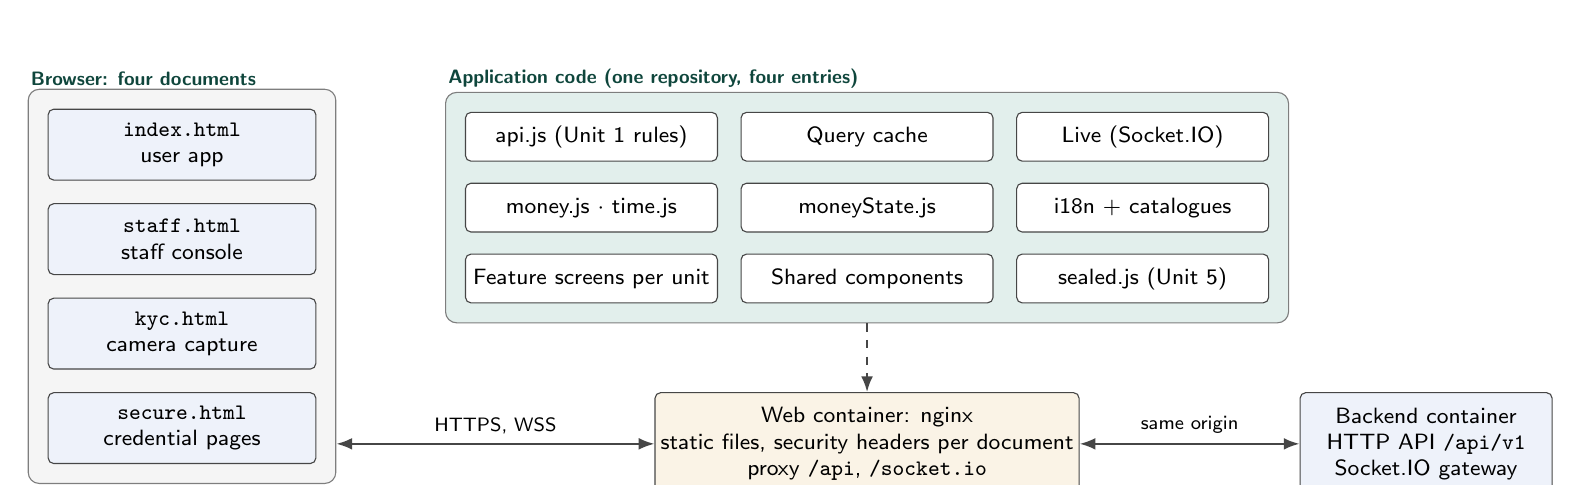
\begin{tikzpicture}[
  font=\sffamily\footnotesize,
  comp/.style={draw=edge, rounded corners=2pt, fill=white, minimum width=3.2cm, minimum height=0.62cm, align=center, inner sep=2pt},
  grp/.style={draw=edge!70, rounded corners=4pt, inner sep=7pt},
  lbl/.style={font=\sffamily\scriptsize\bfseries, text=headcolor, anchor=south west, inner sep=1pt},
  arr/.style={-{Latex[length=2mm]}, draw=edge, thick},
  doc/.style={comp, fill=boxb, minimum width=3.4cm, minimum height=0.9cm}
]
\node[doc] (d1) at (0,4.2) {\texttt{index.html}\\user app};
\node[doc] (d2) at (0,3.0) {\texttt{staff.html}\\staff console};
\node[doc] (d3) at (0,1.8) {\texttt{kyc.html}\\camera capture};
\node[doc] (d4) at (0,0.6) {\texttt{secure.html}\\credential pages};
\begin{scope}[on background layer]\node[grp, fill=boxd, fit=(d1)(d4)] (br) {};\end{scope}
\node[lbl] at (br.north west) {Browser: four documents};
\foreach \n/\x/\y/\t in {m1/5.2/4.3/api.js (Unit 1 rules), m2/8.7/4.3/Query cache, m3/12.2/4.3/Live (Socket.IO),
  m4/5.2/3.4/money.js $\cdot$ time.js, m5/8.7/3.4/moneyState.js, m6/12.2/3.4/i18n + catalogues,
  m7/5.2/2.5/Feature screens per unit, m8/8.7/2.5/Shared components, m9/12.2/2.5/sealed.js (Unit 5)}
  {\node[comp] (\n) at (\x,\y) {\t};}
\begin{scope}[on background layer]\node[grp, fill=boxa, fit=(m1)(m9)] (app) {};\end{scope}
\node[lbl] at (app.north west) {Application code (one repository, four entries)};
\node[comp, fill=boxc, minimum width=4.6cm, minimum height=1.3cm] (ng) at (8.7,0.4) {Web container: nginx\\static files, security headers per document\\proxy \texttt{/api}, \texttt{/socket.io}};
\node[comp, fill=boxb, minimum width=3.2cm, minimum height=1.3cm] (be) at (15.8,0.4) {Backend container\\HTTP API \texttt{/api/v1}\\Socket.IO gateway};
\draw[arr, {Latex[length=2mm]}-{Latex[length=2mm]}] (br.east|-ng.west) -- node[above, font=\sffamily\scriptsize]{HTTPS, WSS} (ng.west);
\draw[arr, {Latex[length=2mm]}-{Latex[length=2mm]}] (ng.east) -- node[above, font=\sffamily\scriptsize]{same origin} (be.west);
\draw[arr, dashed] (app.south) -- (ng.north);
\end{tikzpicture}}
\caption{The web client. One code base builds four documents; the web container serves them with their own headers and forwards the API and the live connection, so browser and API share one origin.}
\label{fig:arch}
\end{figure}

\subsection{Technology}
\begin{dtable}{@{}>{\raggedright\arraybackslash}p{4.0cm}>{\raggedright\arraybackslash}p{2.4cm}>{\raggedright\arraybackslash}p{8.8cm}@{}}
\toprule
\textbf{Library} & \textbf{Version} & \textbf{Use and reason} \\ \midrule \endhead
React, React DOM & 18.3.1 & C-1. Escapes all text by default, which SEC-INP-03 relies on. \\
React Router & 6.26.2 & Routes with lazy-loaded screens; one router per document. \\
TanStack Query & 5.59.0 & Server state: caching, refetch on focus and reconnect, invalidation by live events. Replaces any global store: what the server knows stays the server's. \\
Socket.IO client & 4.8.1 & The live connection (C-1, IF-COM-01). \\
\texttt{@hpke/core} & 1.9.0 & Only in \texttt{secure.html}, through Unit~5's \texttt{sealed.js}; bundled, never from a CDN (SEC-GAM-03). \\
Vite, TypeScript & 7.x, 5.5 & Build (already in the repository); four HTML entries. \\
ESLint & 9.x & NFR-MNT-07, with the security rules of Section~\ref{sec:security}. \\
\bottomrule
\end{dtable}
Exact versions are pinned in \texttt{package-lock.json}. Nothing else is needed. There is no CSS framework, no date library (the browser's \texttt{Intl} does the formatting, Section~\ref{sec:lang}) and no i18n library (the catalogue module is 40 lines). The page budget of NFR-PERF-07 is the reason (Section~\ref{sec:perf}). Styles are CSS modules with design tokens as CSS variables.

% ------------------------------------------------------------------
\section{Application Structure}
\label{sec:structure}

\subsection{Four documents}
A single-page application is one document, and some browser protections apply per document: the Content Security Policy, the Permissions-Policy (which decides whether a page may use the camera), and whether the browser may cache the page. The SRS asks for different settings on different pages (SEC-WEB-02, SEC-GAM-03), so the client is built as four documents, each a Vite entry with its own bundle:
\begin{dtable}{@{}>{\ttfamily\raggedright\arraybackslash}p{2.1cm}>{\raggedright\arraybackslash}p{3.6cm}>{\raggedright\arraybackslash}p{9.5cm}@{}}
\toprule
\textnormal{\textbf{Document}} & \textbf{Paths} & \textbf{Why it is separate} \\ \midrule \endhead
index.html & everything else & The user app. Geolocation is allowed, camera is not. \\
staff.html & \texttt{/staff/*}, \texttt{/admin/*} & Staff code is never sent to users. Staff sessions have their own cookies (I-51) and shorter limits (CP-03), so a staff member signed in to the console is not signed in to the user app in the same browser, and the reverse (FR-OPS-04). \\
kyc.html & \texttt{/account/kyc/*} & The only document allowed to use the camera (SEC-WEB-02, FR-KYC-02). \\
secure.html & \texttt{/secure/orders/\{id\}/\allowbreak credentials}, \texttt{/deliver} & The two credential screens of Unit~5 (SEC-GAM-03): a minimal bundle with \texttt{sealed.js} and nothing else, the strictest policy and \texttt{Cache-Control:} \texttt{no-store}. \\
\bottomrule
\end{dtable}
Moving between documents is a normal page load. Links into a credential screen therefore always load a fresh \texttt{secure.html}, and its policy cannot be loosened by anything that ran on an earlier page.

\subsection{Code layout}
\begin{lstlisting}[language={},basicstyle=\ttfamily\scriptsize]
frontend/
  index.html  staff.html  kyc.html  secure.html     the four entries
  src/
    lib/        api.js money.js time.js moneyState.js live.js i18n.js   (reference modules, unchanged)
    messages/   en/*.json  bn/*.json                 one catalogue file per feature, same keys in both
    shared/     components (Money, DateTime, Deadline, Countdown, ConfirmDialog, StepUpDialog, ...)
    features/   account/ kyc/ listings/ search/ auctions/ checkout/ orders/ delivery/ game/ chat/
                notifications/ disputes/ ratings/ seller/ privacy/      (one folder per unit area)
    staff/      queues/ cases/ admin/                 (only in the staff.html bundle)
    entries/    app.tsx staff.tsx kyc.tsx secure.tsx
\end{lstlisting}
A feature folder holds its routes, screens, query hooks and catalogue keys. It may import \texttt{lib} and \texttt{shared}, but not another feature's internals; a cross-feature link goes through routes. The ESLint import rules check this, and that \texttt{staff/} is imported only by the staff entry.

\subsection{Routes of the user app}
\label{sec:routes}
\begin{dtable}{@{}>{\ttfamily\raggedright\arraybackslash}p{4.6cm}>{\raggedright\arraybackslash}p{2.0cm}>{\raggedright\arraybackslash}p{8.6cm}@{}}
\toprule
\textnormal{\textbf{Path}} & \textbf{Who} & \textbf{Screen (IF-UI)} \\ \midrule \endhead
/, /search & everyone & Home and search with filters (IF-UI-03) \\
/listings/:id & everyone & Listing detail: Buy, or the live auction panel (IF-UI-03) \\
/users/:id & everyone & Public profile with ratings and badges (FR-REV-04, 05) \\
/register, /signin, /reset & guests & IF-UI-01 \\
/sell/new, /sell/:id & verified & Listing creation and editing; game details and ownership proof (IF-UI-03, IF-UI-06) \\
/checkout/:listingId & verified & IF-UI-04 \\
/payments/\allowbreak return/:provider & buyer & Status after the provider's page; never confirms by itself (FR-PAY-02) \\
/orders, /orders/:id & parties & Order view with its tabs: handover or shipment, game account, dispute, chat (IF-UI-05, 06, 07) \\
/messages, /messages/:thread & signed in & Chat (IF-UI-07) \\
/notifications & signed in & Notification centre and preferences (FR-NTF-04, 05) \\
/seller & verified & Seller dashboard (IF-UI-08) \\
/account, /account/security & signed in & Profile; sessions, MFA, password, contact changes (IF-UI-01) \\
/account/payout, /account/privacy & signed in & Payout account (FR-PAY-17); consents, data export, closure (FR-PRV) \\
/help/:topic & everyone & Auction rules, fees, disputes, game-account risks, terms (NFR-CMP-04) \\
\bottomrule
\end{dtable}
\emph{Who} decides only what the client offers; for example, a guest who opens \texttt{/checkout} is sent to sign in. It is not access control. Every request is authorised by the server (SEC-ACC-01), and a screen that receives \texttt{403} or \texttt{404} shows the message for it.

The staff console's routes follow the eight queues of FR-OPS-01 (Unit~7, Section~\ref{sec:console}).
\section{Talking to the Backend}
\label{sec:client}

\subsection{One origin}
The browser loads the documents and calls the API on one origin. In development, Vite's proxy forwards \texttt{/api} and \texttt{/socket.io} to the backend; in the web container, nginx does the same (Section~\ref{sec:build}). All cookies are therefore first-party and \texttt{SameSite=Strict} works, as Unit~1 assumed. The API base is the relative path \texttt{/api/v1}; there is no API address to configure, so the skeleton's \texttt{VITE\_API\_BASE\_URL} goes.

\subsection{The API client}
\label{sec:api}
Every request goes through \texttt{createApi} (\texttt{lib/api.js}, Appendix~\ref{app:code}). It follows Unit~1's rules:
\begin{dtable}{@{}>{\raggedright\arraybackslash}p{3.6cm}>{\raggedright\arraybackslash}p{11.6cm}@{}}
\toprule
\textbf{Rule} & \textbf{What the client does} \\ \midrule \endhead
Tokens (SEC-SES-03) & None in reach of scripts. Requests use \texttt{credentials: 'same-origin'}; the browser sends the HttpOnly cookies. The client never sets an \texttt{Authorization} header (tested in Chromium). \\
CSRF (SEC-SES-04) & On \texttt{POST}, \texttt{PUT}, \texttt{PATCH} and \texttt{DELETE}, \texttt{X-CSRF-Token} is copied from the readable \texttt{\_\_Host-tb\_csrf} cookie. It is read on each attempt, so a refresh's new cookie is used at once. \\
Expired access token & On \texttt{401}, the client refreshes once and retries the request once, with the same headers. If the refresh is refused, or the retry is \texttt{401} again, the session has ended: the app clears its cache and shows ``You have been signed out''. \\
One refresh for all tabs & Refreshes are serialised across tabs with the Web Locks API (lock \texttt{tb-refresh}). A tab that obtains the lock first checks whether another tab has already refreshed, and if so retries without refreshing. A \texttt{409} from the refresh endpoint (``rotated a moment ago'', Unit~1 DV-4) is retried after 300~ms. \\
Step-up (SEC-AUTH-08) & A request declared with a step-up action (for example \texttt{payout.change}) first opens the step-up dialog. The dialog calls \texttt{/auth/step-up/start} and \texttt{/verify}; the grant goes in \texttt{X-Step-Up}. The grant is used once and kept only in memory. \\
Idempotency & Requests that create something (an order, a payment, a bid, a dispute, a listing) carry an \texttt{Idempotency-Key} chosen once per user action and kept across the retry after a refresh. The server's use of it is I-51. \\
Errors (DC-3) & Problem documents become \texttt{ApiError} with status, type, correlation id, field errors and \texttt{Retry-After}. Each maps to one message (table below). \\
\bottomrule
\end{dtable}

\textbf{Checking for another tab's refresh.} The first version of the client recorded each refresh time in \texttt{localStorage}. A tab that saw a time later than its own failed request skipped the refresh. The browser test showed that this was not enough: in 5 of 10 runs, three tabs racing after an expiry produced two refreshes. The reason is that \texttt{localStorage} writes reach other tabs with a delay, so a tab may not yet see the time another tab wrote. The second refresh was harmless (Unit~1 rotates the token again), but it was not the behaviour Unit~1 designed for. The client now uses the \texttt{localStorage} time only as a quick hint. Inside the lock, before refreshing, it sends one \texttt{GET /me}. The browser attaches whatever cookies it currently holds, and the cookie store is shared by all tabs at once. If \texttt{/me} succeeds, another tab has refreshed and the request is simply retried. With this change, 30 racing rounds over 6 runs gave one refresh each. The cost is one extra request per tab every 15~minutes (CP-01).

\textbf{Errors and messages.} Messages are generic, as SEC-INP-06 requires, and come from the catalogue:
\begin{dtable}{@{}>{\raggedright\arraybackslash}p{2.6cm}>{\raggedright\arraybackslash}p{6.4cm}>{\raggedright\arraybackslash}p{6.2cm}@{}}
\toprule
\textbf{Response} & \textbf{Shown} & \textbf{Then} \\ \midrule \endhead
network failure & ``We could not reach TrustBazaar \dots'' & Queries retry on reconnect; a state change is never retried automatically. \\
401 (after refresh) & ``You have been signed out \dots'' & Cache cleared; sign-in page, returning to the same path afterwards. \\
403 step-up & ``\dots{} enter the code we sent \dots'' & The step-up dialog. \\
403 other, 404 & Not allowed; no longer exists & No retry. \\
409 & ``This changed while you were looking at it \dots'' & The screen's queries are refetched, so the user sees the new state before trying again. \\
422 & Field errors next to their fields & Focus moves to the first field in error. \\
429 & ``Try again in \{seconds\} seconds'' & The button stays disabled for \texttt{Retry-After}. \\
5xx & ``\dots{} quote reference \{ref\}'' & The correlation id, so support can find the log entry. \\
\bottomrule
\end{dtable}

\textbf{Sent once.} Every button that changes state is disabled from the click until the answer, and the request carries its idempotency key. A double click, a retry after a refresh, or a request repeated after a lost response therefore cannot pay twice or bid twice. The database rules of Units~2 and~3 stay the final barrier.

\subsection{Server state}
\label{sec:cache}
What the server knows (listings, orders, threads, the account) is held in TanStack Query's cache and nowhere else. A screen reads through a query hook and changes things through a mutation that invalidates the affected queries. Query keys follow the API paths, for example \texttt{['orders', id]} and \texttt{['auctions', id, 'state']}. Freshness depends on how fast the data changes and how much a stale view costs:
\begin{dtable}{@{}>{\raggedright\arraybackslash}p{5.2cm}>{\raggedright\arraybackslash}p{2.6cm}>{\raggedright\arraybackslash}p{7.4cm}@{}}
\toprule
\textbf{Data} & \textbf{Stale after} & \textbf{Refreshed also} \\ \midrule \endhead
Order, escrow, handover, game handover, dispute & 0 & On focus, on reconnect, on every notification about that order. \\
Auction state & live & The live feed (Section~\ref{sec:live}); \texttt{/state} on open, on reconnect and every 60~s. \\
Search results, listings & 30 s & On focus. \\
Categories, areas, games, meetup points & 1 hour & --- \\
Own account (\texttt{/me}), KYC status & 0 & After sign-in, step-up and KYC submission. \\
\bottomrule
\end{dtable}
After sign-out or a \texttt{401}, the whole cache is cleared, so one user's data never shows to the next user of a shared phone.

\subsection{The live connection}
\label{sec:live}
Each tab opens one Socket.IO connection to \texttt{/socket.io} after sign-in. Unit~1 authenticates it with the session cookie when it opens (SEC-SES-07). The server places it in the user's room. The client joins an auction room while an auction page is open.
\begin{dtable}{@{}>{\ttfamily\raggedright\arraybackslash}p{3.3cm}>{\raggedright\arraybackslash}p{1.6cm}>{\raggedright\arraybackslash}p{10.3cm}@{}}
\toprule
\textnormal{\textbf{Event}} & \textbf{From} & \textbf{Client handling} \\ \midrule \endhead
auction.state & Unit 3 & \texttt{AuctionFeed.apply}: whole state with a sequence number; an older or repeated one is dropped. Its \texttt{serverTime} feeds the clock. \\
auction.closed & Unit 3 & Final result; the panel shows sold or unsold, and the winner is taken to the order. \\
auction.outbid & Unit 3 & A notice to the previous leader, and a refetch of \texttt{my-status}. \\
chat.message & Unit 6 & \texttt{ChatThread.receive}: appended if it is the next number; our own message is recognised by its client id; a gap triggers \texttt{GET /threads/\{id\}/messages?after=}. \\
notification.new & Unit 6 & Unread count; invalidates the queries of the object it names (I-55). \\
\bottomrule
\end{dtable}
\textbf{Reconnection} (IF-COM-02). Socket.IO reconnects with a growing delay (DV-57). Live messages may have been missed in between, so after a reconnection the client refetches the state of every open auction, resyncs every open thread from its last sequence number, and invalidates the order queries. Phones that slept are handled the same way, because the connection drops. If a reconnection is refused because the access token expired, the client refreshes through \texttt{api.js} and connects again.

\textbf{Guests} do not get the live connection (Unit~3); the auction page polls \texttt{/state} every DV-19 and shows ``Sign in for live updates''.

\textbf{Ordering, tested.} The auction feed keeps only newer states in any arrival order. In the chat test, 200 messages arrive shuffled with a fifth of them lost; after resyncs the thread is complete and in order (Appendix~\ref{app:tests}).

\subsection{The server clock and countdowns}
\label{sec:clock}
Auction ends, payment windows, takeover windows and dispute deadlines are counted down on the server's clock, because a phone's clock can be minutes wrong (FR-AUC-01). \texttt{ServerClock} (\texttt{lib/time.js}) estimates the difference from the \texttt{serverTime} field:
\begin{itemize}[nosep]
  \item A response to a request sent at $s$ and received at $r$, carrying server time $T$, bounds the offset: it lies between $T - r$ and $T - s$.
  \item A live message gives only the lower bound $T - r$, because it may have been delayed.
  \item The estimate is the middle of the intersection of the last 8 samples (DV-55), or its lower bound if no response has given an upper bound. A delayed message therefore never moves the estimate the wrong way. If the samples contradict each other, the device clock has jumped, and only the newest sample is kept.
\end{itemize}
One timer per tab ticks once a second and updates every visible countdown. Countdowns always show the time remaining according to the server's clock, so a bid placed in the last seconds is judged by the same clock the user saw. The server alone decides whether a bid arrived in time (Unit~3), and the screen says so near the end: ``The auction ends on the server's clock; a bid sent in the last second may arrive too late.''
\section{Screens}
\label{sec:screens}
Each screen is listed with what it must show, what it calls, and the rules the SRS or an earlier unit set for it. Shared components keep the rules in one place: \texttt{<Money>}, \texttt{<DateTime>} and \texttt{<Deadline>} format through \texttt{lib/} (Section~\ref{sec:lang}); \texttt{<ConfirmDialog>} shows an action's consequence (IF-UI-10); \texttt{<SimulatedBanner>} appears on every payment and courier screen (NFR-CMP-05); \texttt{<StepUpDialog>} asks for the OTP.

\subsection{Account and sign-in (IF-UI-01)}
\begin{dtable}{@{}>{\raggedright\arraybackslash}p{3.0cm}>{\raggedright\arraybackslash}p{5.4cm}>{\raggedright\arraybackslash}p{6.8cm}@{}}
\toprule
\textbf{Screen} & \textbf{Calls (Unit 1)} & \textbf{Rules shown} \\ \midrule \endhead
Register & \texttt{/auth/register}, \texttt{/verify}, \texttt{/resend} & Age confirmation and the privacy notice before submit (FR-PRV-01); OTP resend disabled for \texttt{Retry-After}. \\
Sign in & \texttt{/auth/signin}, \texttt{/signin/mfa} & One error text for every failure (Unit~1 does not reveal which accounts exist); the growing delay shown as a countdown. \\
Reset & \texttt{/auth/password/forgot}, \texttt{/reset} & The same answer whether or not the account exists. \\
Security & \texttt{/auth/sessions}, \texttt{DELETE /auth/sessions/\{id\}}, \texttt{/end-others}, MFA, password and contact changes & Sessions with device, area and last use; ``this device'' marked. Changes use step-up. After a password change, other sessions are shown as ended. \\
Privacy & \texttt{/me/consents}, \texttt{/me/data-export}, \texttt{/me/close} & What closing removes and keeps (FR-ACC-11) before the step-up; the export link's 7 days (DV-49). \\
\bottomrule
\end{dtable}

\subsection{KYC wizard (IF-UI-02, NFR-USE-02)}
The wizard is \texttt{kyc.html}, the only document allowed the camera. Before any capture it states what is needed: an NID or passport, both sides, a live selfie, good light, and no glare. Then it guides each capture with \texttt{getUserMedia} and shows the image for retaking. The liveness step shows the random action from \texttt{/kyc/liveness-challenge}. The status (\texttt{/kyc/status}) is shown at the top of every step, with the rejection reason when there is one. Images are sent once, at the end, to \texttt{/kyc/submissions}. They are kept only in memory until then, never in browser storage. Files already uploaded are shown through Unit~1's signed links only. When the camera is refused, the wizard explains how to allow it and offers a file upload for the documents, though not for the selfie (FR-KYC-02).

\subsection{Listings, search and the auction panel (IF-UI-03, NFR-USE-01)}
\textbf{Create and edit} (\texttt{/sell}): category from \texttt{/categories}, where prohibited ones show their policy (FR-LST-10); photos uploaded one by one with progress, up to CP-33; the area chosen on a list, or found with the Geolocation API after a button press, with the list as the fallback (IF-SW-08). Before publishing, the screen shows the commission that will be deducted from the payout (CP-25, FR-MON-01). It also states FR-LST-07's limit: after the first bid or order, only clarifications can be added, and an auction's starting price, reserve and duration never change after publishing. A listing sent to review says so.

\textbf{Search} (\texttt{/search}): filters in the URL, so a search can be shared and the back button works; cursor pages appended with a ``Show more'' button rather than endless scrolling, so the footer and its help links stay reachable; distance shown in whole kilometres (Unit~4).

\textbf{The auction panel} on the listing page:
\begin{itemize}[nosep]
  \item current price, bid count, masked leader, reserve met or not, and the countdown on the server's clock;
  \item the minimum next bid (price plus the increment, CP-08), and an input parsed by \texttt{parseTaka}, which accepts Bangla digits. An amount below the minimum is explained before sending;
  \item ``Your maximum'' and ``You are leading'', from \texttt{my-status}, shown only to the bidder; a proxy bid explained in one sentence (\texttt{confirm.proxy\_bid});
  \item the rules (increment, proxy bidding, reserve, anti-sniping) in a panel that opens in place, so the bidder never leaves the page (NFR-USE-01);
  \item the masked bid history (FR-AUC-13);
  \item after ``Place bid'': the confirmation (\texttt{confirm.place\_bid}), then \texttt{POST /auctions/\{id\}/bids} with an idempotency key. If the price moved meanwhile, the answer is shown with the new minimum. Live updates continue while the dialog is open, and the dialog shows the new price if it changes.
\end{itemize}
Price changes are announced to screen readers in a polite live region at most every 5 seconds, plus at once when the user is outbid. The countdown itself is not announced every second; it is announced at 5 minutes and 1 minute.

\subsection{Checkout and payment (IF-UI-04)}
A fixed-price checkout starts with \texttt{POST /orders}, which reserves the item (Unit~2); an auction win already has its order. The checkout shows one total, with the item price and the delivery fee beneath it, the fulfilment method, the payment method and the fee disclosure. The fee is the platform's commission, paid by the seller; the buyer pays the total shown and nothing more. Each fulfilment option shows its fee from the binding quote (Unit~4, DV-23), and the quote's expiry as a countdown. ``Pay'' opens \texttt{confirm.buy\_now} and calls \texttt{POST /orders/\{id\}/payments} with an idempotency key.

The answer is the provider's page. The client follows it only if its host is on the list of providers: bKash, Nagad and Stripe sandboxes, and the mock provider (Section~\ref{sec:security}). After the provider, \texttt{/payments/return/:provider} shows only the order's status. It never treats the return as payment (FR-PAY-02). It polls \texttt{GET /orders/\{id\}} every 2~seconds for up to 30~seconds, and then says ``We are still waiting for the payment provider. We will notify you'' (NFR-PERF-06 expects 5~seconds). The simulated-payments banner is on every payment screen.

\subsection{The order view (IF-UI-05, NFR-USE-07)}
\label{sec:orderview}
One screen for buyer and seller, built from \texttt{GET /orders/\{id\}} and the unit tabs. From top to bottom:
\begin{enumerate}[nosep]
  \item \textbf{Where the money is}, in one sentence from \texttt{describeMoney} (Section~\ref{sec:moneystate}).
  \item \textbf{Every deadline that applies}, each as a time and a countdown (NFR-USE-08): payment window, fulfilment deadline, meetup time, auto-release or the end of the protection period, dispute window, and the seller's response deadline in a dispute.
  \item \textbf{What can be done now}, and only that. Each action shows its consequence first: confirm receipt (\texttt{confirm.confirm\_receipt}), open a dispute, ask to cancel; for the seller, cancel (\texttt{confirm.seller\_cancel}, with the strike). Only actions the server's state allows are offered, and the server checks again.
  \item \textbf{Fulfilment}: the handover tab or the shipment tab (Unit~4), or the game-account tab (Unit~5).
  \item \textbf{Chat} with the other party (Unit~6) and, after the order closes, the rating (Unit~7).
\end{enumerate}

\textbf{Handover code} (Unit~4). The buyer sees the code with its instruction, \texttt{confirm.\allowbreak share\_handover\_code}: ``Give this code to the seller only after you have checked the item.'' The code is large, readable aloud digit by digit, and hidden behind a ``Show code'' button, so it does not show on a screen held up at a meetup. The seller's entry screen says ``Hand over the item only after the buyer gives you the code'' and shows the attempts left before the lock. Meetup proposals list the curated points with a map link. Map links are offered only for these public points, never for a user's address (Unit~4). A shipment shows its status history and the ``simulated'' banner.

\subsection{Game accounts (IF-UI-06, NFR-USE-03)}
\textbf{Seller, before sale}: game details, then the ownership-code screen. The code is shown with where to place it in that game (from \texttt{/games}) and its expiry countdown; then the screenshot upload, and the proof's status.

\textbf{Buyer, before purchase}: the disclosure (FR-GAM-05), acknowledged by version. The checkout first checks that this browser has Web Crypto and IndexedDB (Unit~5, AS-5). If not, it says the purchase needs a browser that supports them and stops. It also tells the buyer: ``Use this same browser on this device to open the credentials. If you clear its data or change device, you can ask the seller to send them again once.''

\textbf{The two credential screens} are \texttt{secure.html} (Section~\ref{sec:security}):
\begin{itemize}[nosep]
  \item \textbf{Deliver} (seller): the buyer's key fingerprint, in Unit~5's five groups of four, to compare if the parties wish; the credential fields with autocomplete and spell-checking off; then \texttt{sealed.js} seals the credentials in the page and sends only the ciphertext. Nothing typed is kept after sending.
  \item \textbf{Credentials} (buyer): opens the ciphertext with the key in IndexedDB, shows the credentials, and next to them the takeover checklist. Each step is confirmed by its own button. The remaining takeover window (CP-23) is shown as a countdown, and the date the protection period ends beside it (NFR-USE-03). ``The credentials do not work'' is offered until the recovery e-mail step is confirmed (FR-GAM-14).
\end{itemize}
On the order view, early release asks for step-up and states \texttt{confirm.release\_early}.

\subsection{Chat (IF-UI-07)}
\begin{itemize}[nosep]
  \item Text is rendered as text only (SEC-INP-03). A web address in a message is shown as plain text, not a link (Unit~6).
  \item A message flagged by Unit~6 shows its warning to both parties, under the message: off-platform payment, contact details, or login details. For login details, the warning points the seller to the sealed handover.
  \item Each message gets a random client id when it is typed, and keeps it for its resends; it shows ``sending'' until the server's copy arrives (\texttt{ChatThread}).
  \item Block and report are on every thread. Images are shown through signed links, with their size limited in the layout.
\end{itemize}

\subsection{Disputes and ratings (Unit 7)}
The dispute flow starts from the order view, and only the types allowed now are offered; the server answers that through Unit~7. The flow takes a type, a description of at least 20 characters, and up to 10 files (CP-33), and shows \texttt{confirm.open\_dispute}. The dispute tab then shows the status, the seller's response deadline and the decision target as countdowns, both parties' statements, and, after the decision, the outcome and its reason. Withdrawing shows \texttt{confirm.withdraw\_dispute} with the new auto-release time. The rating form appears after the order closes, with the end of the rating window and of the edit period (CP-39).

\subsection{Seller dashboard (IF-UI-08)}
Listings by state, orders needing action (with their deadlines first), the payout account and its check status, payouts and statements; for Pro Sellers, sales analytics (sales, views to orders, average price, by month). Figures come from the server; the dashboard computes nothing about money.

\subsection{Staff console (IF-UI-09)}
\label{sec:console}
\texttt{staff.html}, signed in with staff accounts only, with MFA (Unit~1).
\begin{itemize}[nosep]
  \item \textbf{Queues}: the eight queues of FR-OPS-01 (IF-UI-09 names five; the console shows all eight, Unit~7). Each queue is ordered oldest first, with overdue items on top and each item's age.
  \item \textbf{Claim}: a case opens only after a claim; a conflict refusal (FR-OPS-06) is shown as its message.
  \item \textbf{Case file}: personal data is masked by default (SEC-ACC-05); ``Show'' asks for a reason, which the server logs. KYC images and evidence open through signed links that expire (CP-31). The chat thread of the case is shown only when the case holds it.
  \item \textbf{Actions}: only the actions of FR-OPS-02, each with a required reason. A dispute decision shows the outcome preview (the exact split from Unit~2) and, at CP-30, ``This decision needs a second operator's approval''.
  \item \textbf{Approvals}: the open four-eyes proposals for the staff member's role, never their own.
  \item \textbf{Administrators}: staff accounts; the parameter editor, which shows every broken rule at once (Unit~7's \texttt{config\_violations}); emergency switches with four-eyes; reference data (games, areas, meetup points, screening and detection terms); the audit log, read-only.
\end{itemize}
The console has no ``edit user'', ``edit order'' or ``edit payment'' screen, because none exists in the API (FR-OPS-02). The console shows staff sessions' shorter idle limit (CP-03) as a warning a minute before sign-out.

\subsection{Consequences before confirmation (IF-UI-10)}
Every action that moves money, ends a right or cannot be undone opens \texttt{<ConfirmDialog>} with its consequence message, filled with the real amounts and times. The confirm button names the action and its amount (``Release Tk 12,550 to the seller'') rather than saying ``OK''. The reference catalogue has the nine messages these actions need: confirm receipt, early release, opening and withdrawing a dispute, seller cancellation, bids, proxy bids, buying and the handover code. A test checks that each exists in both languages with the same placeholders.
\section{Language, Money and Time}
\label{sec:lang}

\subsection{Bangla and English (NFR-USE-04)}
\begin{itemize}[nosep]
  \item \textbf{Choice.} A switch in the header of every page, at any time. A signed-in user's choice is saved in their notification preferences (Unit~6), so notices use the same language. A guest's choice is kept in \texttt{localStorage}. With no choice yet, the app uses Bangla if the browser prefers Bangla, and English otherwise (DV-58). \texttt{<html lang>} follows the choice, so screen readers pronounce correctly; text from the other language inside a page (a user's listing title, say) is not marked up, because its language is not known.
  \item \textbf{Catalogues.} One file per feature and language, loaded with the feature's code, with the same keys in both languages (tested). Messages are plain text with \texttt{\{name\}} placeholders, filled with text that is already formatted (money, times). No message contains markup (tested), so a translation can never inject HTML. In development, a missing key or placeholder throws; in production it shows the key, which the catalogue test makes impossible to ship.
  \item \textbf{Server text.} Category names, games and areas arrive in both languages from the API. Notification titles arrive in the user's language (Unit~6). Error messages are always the client's own, chosen by status (Section~\ref{sec:api}).
  \item \textbf{Bangla text} in the reference catalogue was written for this design. The team should review it before release, and a native speaker should review the full catalogue.
  \item \textbf{Font.} Noto Sans Bengali, self-hosted as WOFF2 with \texttt{font-display: swap}, and preloaded only when the language is Bangla. The Latin text uses the system font.
\end{itemize}

\subsection{Money}
\label{sec:money}
Amounts arrive as integer poisha and stay integers: \texttt{formatMoney} works on \texttt{BigInt}, so an amount is never rounded on its way to the screen (tested above $2^{53}$ poisha). The display uses the taka sign before the amount and lakh grouping (12,34,567) in both languages, with Bangla digits in Bangla. A single price drops ``.00''; the lines of a breakdown and a receipt always show two decimals, so they line up (DV-59). Input goes through \texttt{parseTaka}. It accepts Bangla or ASCII digits, group commas in either the lakh or the Western style, an optional taka sign, ``Tk'' or ``BDT'', and up to two decimals. It never passes through a floating-point number, so 0.1 taka is exactly 10 poisha. Every refusal has a reason the form can show (empty, wrong format, too many decimals, too large); limits such as the minimum bid are the server's, and the form shows them before sending.

\subsection{Dates, times and deadlines (NFR-USE-08)}
Every time is formatted in \texttt{Asia/Dhaka}, whatever the device's zone, with weekday, date, month, year and time: ``Tue 20 Oct 2026, 6:00 pm''. The tests pass with the device in four other zones, and Chromium set to New York produces the same text as Node. The day period in Bangla is set by the module (\emph{p\=urb\=ahna}, \emph{apar\=ahna}), because browsers' locale data differ here: Node's prints ``PM'' inside Bangla text. Every deadline is shown as a time and a countdown: ``Tue 20 Oct 2026, 6:00 pm (in 2 days 1 h)''. Countdowns use days and hours above a day, hours and minutes above an hour, and minutes and seconds below; they never show 0:00 before the end. In the last 5 minutes they turn urgent, shown by both colour and text.

\subsection{The money state in plain language (NFR-USE-07)}
\label{sec:moneystate}
\texttt{describeMoney(order, role)} chooses one of nine sentences for each role from the order's status, escrow state, release policy and deadlines, and \texttt{renderMoney} fills it. The SRS's example is reproduced word for word by the test:
\begin{quote}\small
``Your payment is held by TrustBazaar. The seller is paid when you confirm receipt, or automatically on Tue 20 Oct 2026, 6:00 pm unless you open a dispute.''
\end{quote}
\begin{dtable}{@{}>{\raggedright\arraybackslash}p{4.2cm}>{\raggedright\arraybackslash}p{11.0cm}@{}}
\toprule
\textbf{State} & \textbf{Buyer sees (the seller has a matching sentence)} \\ \midrule \endhead
awaiting payment & Nothing has been charged yet. Pay by \{due\} to keep this order. \\
held, before delivery & Your payment of \{amount\} is held by TrustBazaar. The seller must hand the item over by \{due\}, or you get a full refund. \\
held, after delivery & The SRS sentence above. \\
held, game protection & Your payment is held until the protection period ends on \{at\}. If the seller takes the account back before then, open a dispute. \\
frozen (dispute) & Your payment of \{amount\} is frozen while TrustBazaar reviews your dispute. Nobody is paid until it is decided. \\
released, refunded, partially refunded & Who got how much, and when. \\
\bottomrule
\end{dtable}
The sentence is chosen from the server's fields only; the client never infers a state the server has not reported. An unknown escrow state throws instead of showing a guess (tested).

% ------------------------------------------------------------------
\section{Accessibility and Small Screens}
\label{sec:a11y}
\textbf{Small screens} (NFR-USE-05). The layout is designed for small screens first, as one column, and is checked at 320 CSS pixels, the WCAG reflow width, which is narrower than the SRS's 360. Tables in the console and the seller dashboard become stacked cards below 600 pixels. Long unbroken strings (order references, fingerprints, links in chat) may wrap anywhere. The planned end-to-end run visits every route at 360 by 740 and fails if the page scrolls sideways (Section~\ref{sec:testing}).

\textbf{WCAG 2.2 AA} (NFR-USE-06). The choices that matter most for this site:
\begin{itemize}[nosep]
  \item native elements first: buttons, links, form controls, \texttt{<dialog>} for confirmations, with focus moved into the dialog and back when it closes;
  \item every control reachable and usable by keyboard; a visible focus ring of at least 2 pixels and 3:1 contrast;
  \item targets of at least 24 by 24 pixels (2.5.8), and 44 for the main actions (Pay, Place bid, Confirm receipt);
  \item text contrast of at least 4.5:1 from the design tokens; no state shown by colour alone (escrow, urgency and warnings always have text or an icon with a label);
  \item every field with a visible label; errors next to their field and in a summary at the top, linked to the field, with focus moved to the summary;
  \item live regions only where a change matters: bids and outbid notices (polite, at most every 5 seconds), chat messages, step-up and errors. Countdowns are \texttt{role="timer"} and are not read out every second; they are announced at 5 minutes and 1 minute;
  \item reduced motion respected; no content that flashes;
  \item time limits (2.2.1): auctions are a real-time event, which WCAG exempts. A checkout quote or a payment window that expires can be started again from the same screen.
\end{itemize}
The planned end-to-end run checks every route with axe-core and fails on any serious or critical issue (Section~\ref{sec:testing}). Manual checks with a screen reader (TalkBack on Android, NVDA on Windows) cover the bid, checkout, order and handover-code flows.

% ------------------------------------------------------------------
\section{Security}
\label{sec:security}

\subsection{Security headers per document}
The web container sets the headers of the four documents; the backend sets its own on API responses (Unit~1, DC-11). The reference configuration is \texttt{docs/design/web/container/} (Appendix~\ref{app:code}). It was run in nginx~1.24 and checked from Chromium (Section~\ref{sec:testing}).
\begin{dtable}{@{}>{\raggedright\arraybackslash}p{2.6cm}>{\raggedright\arraybackslash}p{12.6cm}@{}}
\toprule
\textbf{Header} & \textbf{Value and reason} \\ \midrule \endhead
CSP, user app and console & \texttt{default-src 'self'; script-src 'self'; style-src 'self'; img-src 'self' data: blob:; connect-src 'self'; object-src 'none'; frame-src 'none'; base-uri 'none'; form-action 'self'; frame-ancestors 'none'; require-trusted-types-for 'script'; trusted-types 'none'}. No inline script, no \texttt{eval}, no third-party origin (SEC-WEB-01). The payment providers are reached by full-page redirect, not framed or scripted, so they need no place in the policy and SEC-WEB-01's exception is not used. \\
CSP, KYC & The same, with \texttt{media-src 'self' blob:} for the camera preview. \\
CSP, credentials & \texttt{default-src 'none'} and only \texttt{'self'} for scripts, styles, images, fonts and connections; \texttt{form-action 'none'} (SEC-GAM-03). \\
Trusted Types & With \texttt{trusted-types 'none'}, any attempt to put an HTML string into the page through \texttt{innerHTML} or a similar sink throws. That backs SEC-INP-03 in the browser itself. React renders text through DOM methods and works under it (tested); \texttt{dangerouslySetInnerHTML} would fail, and is also banned by ESLint. \\
Permissions-Policy & Camera only in \texttt{kyc.html}; geolocation only in the user app; microphone, payment, USB, serial, Bluetooth and the motion sensors nowhere (SEC-WEB-02). \\
Cache-Control & HTML \texttt{no-cache}, so a new release reaches every user on their next page load; the console, KYC and credential pages \texttt{no-store}; hashed assets cached for a year. \\
Others & \texttt{X-Content-Type-Options: nosniff}; \texttt{Referrer-Policy: same-origin} (\texttt{no-referrer} on the console and credentials); \texttt{Cross-Origin-Opener-Policy} and \texttt{-Resource-Policy: same-origin}. HSTS is set by the TLS front (Unit~9). \\
\bottomrule
\end{dtable}
\textbf{Development.} Vite's development server injects an inline script for hot reloading, so these policies apply to the production build only. The end-to-end tests run against the production build in the container, never the development server.

\textbf{Geolocation per document.} SEC-WEB-02 allows the camera and geolocation ``only on the pages that need them''. A single-page app cannot narrow a permission below its document. The camera has a document of its own, as the requirement intends. Geolocation is allowed in the user app, where search and listing creation use it, and is requested only when the user presses ``Use my location''. An SRS clarification states this (I-58).

\subsection{Other client-side rules}
\begin{itemize}[nosep]
  \item \textbf{Text only} (SEC-INP-03). User text is rendered as React text. ESLint forbids \texttt{dangerouslySetInnerHTML} and direct \texttt{innerHTML}, and Trusted Types enforces the same rule in the browser. Links in user text are not made clickable.
  \item \textbf{Leaving the site.} The client follows a payment redirect only to an exact, configured provider host over HTTPS, or to a same-origin path for the mock provider (\texttt{checkProviderRedirect}, tested against look-alike hosts, other ports, credentials in the URL, \texttt{javascript:} and protocol-relative URLs). The host list comes from Unit~2's adapter settings at build time.
  \item \textbf{Storage.} Browser storage holds only: the language choice for guests, the time of the last token refresh, and, in IndexedDB, the buyer's non-extractable game-account key (Unit~5). ESLint allows \texttt{localStorage} only in the modules that keep those. No personal data, no draft containing personal data, and no API response is stored.
  \item \textbf{Masking} (SEC-ACC-05). The console shows the masked values the API returns. ``Show'' sends a reason, and only the server's answer, which is logged, contains the full value.
  \item \textbf{Dependencies.} Exact versions in the lock file; \texttt{npm audit} in CI; no script or style from another origin, so SEC-WEB-04's integrity hashes have nothing to apply to.
  \item \textbf{Simulated services} (NFR-CMP-05). \texttt{<SimulatedBanner>} on checkout, payment return, shipment and payout screens, in both languages.
\end{itemize}

% ------------------------------------------------------------------
\section{Performance}
\label{sec:perf}
NFR-PERF-07 asks for the largest contentful paint within 2.5~seconds on the home, listing and checkout pages, on 4G and a mid-range phone.
\begin{itemize}[nosep]
  \item \textbf{Code splitting.} Each route is a lazy chunk. The first load of the user app carries React, the router, the query cache, \texttt{lib/} and the page's own chunk; the live connection is loaded after the first paint. The budget is 170~KB of compressed JavaScript for the first load of these three pages (DV-53), to be checked in CI from the build's chunk sizes.
  \item \textbf{The largest paint} on a listing page is its first photo. It uses Unit~3's 1600-pixel image with the 400-pixel thumbnail as \texttt{srcset} alternatives, explicit width and height (no layout shift), and \texttt{fetchpriority="high"}. Other photos and search thumbnails load lazily.
  \item \textbf{Data.} The listing page renders from one request (\texttt{GET /listings/\{id\}}, which includes the auction state); search results come from one request with cursor pages.
  \item \textbf{Measurement} (planned). Lighthouse runs in CI against the production build, with its mobile profile (simulated 4G and a slowed processor), on the three pages, and fails above 2.5~seconds.
\end{itemize}
The live paths are measured end to end by Units~3 and~6 (NFR-PERF-03, 04). The client adds one state update and a render, which takes milliseconds.

% ------------------------------------------------------------------
\section{Build and the Web Container}
\label{sec:build}
\begin{itemize}[nosep]
  \item \textbf{Vite.} Four HTML entries (\texttt{build.rollupOptions.input}); hashed file names under \texttt{/assets/}; target ES2020, matching the supported browsers: the last two versions of Chrome, Edge, Firefox and Safari, and Chrome and Samsung Internet on Android. The development server proxies \texttt{/api} and \texttt{/socket.io} (with WebSocket) to the backend.
  \item \textbf{Configuration.} Only build-time values that are not secret: the provider host list and the feature flags known at build time. Parameters (fees, windows, limits) are never built in. They come from the API, which reads Unit~7's current version (NFR-MNT-06).
  \item \textbf{Dockerfile.} Two stages: \texttt{node:\allowbreak 20-alpine} runs \texttt{npm ci} and \texttt{npm run build}; \texttt{nginx:\allowbreak 1.27-alpine} serves \texttt{dist/} with the reference configuration and proxies to \texttt{backend:3000}. This is the web container of NFR-MNT-01, and it replaces the current Dockerfile, which runs the development server. Developers still use \texttt{npm run dev} outside Docker.
  \item \textbf{Health.} \texttt{GET /healthz} answers from nginx without touching the backend, for Compose's health check (Unit~9).
\end{itemize}
\section{Parameters}
\textbf{SRS parameters shown or used by the client:} every deadline parameter through the server's values (CP-10, CP-11, CP-17 to CP-24, CP-39); CP-01 and CP-03 (session lengths, for the refresh and the console's warning); CP-08 (shown as the minimum next bid, from the server); CP-25 (commission shown to sellers); CP-31 (signed links); CP-33 (upload limits checked before sending); CP-35 (limits answered by \texttt{429}). None is built into the client (NFR-MNT-06).

\textbf{Design values introduced} (continuing DV-1 to DV-52):
\begin{dtable}{@{}>{\bfseries}p{1.3cm}>{\raggedright\arraybackslash}p{4.4cm}>{\raggedright\arraybackslash}p{4.8cm}>{\raggedright\arraybackslash}p{4.4cm}@{}}
\toprule
\textnormal{\textbf{ID}} & \textbf{Value} & \textbf{Default} & \textbf{Reason} \\ \midrule \endhead
DV-53 & First-load JavaScript, home, listing and checkout & at most 170 KB compressed & NFR-PERF-07 on 4G. \\
DV-54 & Countdowns & tick 1 s; urgent in the last 5 min; announced at 5 and 1 min & Readable without flooding screen readers. \\
DV-55 & Server clock & last 8 samples; \texttt{/state} again every 60 s on an auction page & Corrects drift and sleeping devices. \\
DV-56 & Cache freshness & orders and money 0; search 30 s; reference data 1 h & A stale money view costs trust. \\
DV-57 & Live reconnection & 0.5 s doubling to 10 s, with random spread & Many phones reconnecting at once do not arrive together. \\
DV-58 & Default language & Bangla if the browser prefers it, otherwise English & Most users are in Bangladesh. \\
DV-59 & Money decimals & dropped when zero for single prices; always two in breakdowns & Clean prices; aligned sums. \\
DV-60 & After the payment provider & ask every 2 s for up to 30 s & NFR-PERF-06 is 5 s; the rest covers slow callbacks. \\
\bottomrule
\end{dtable}

\section{Testing}
\label{sec:testing}
\begin{dtable}{@{}>{\raggedright\arraybackslash}p{3.2cm}>{\raggedright\arraybackslash}p{12cm}@{}}
\toprule
\textbf{Level} & \textbf{Cases} \\ \midrule \endhead
Reference modules (done) & 46 tests with Node's test runner (\texttt{npm run test:unit}). API client: CSRF on state changes only; one refresh and one retry with the same idempotency key; ten failing requests, one refresh; another tab's refresh reused, also when its \texttt{localStorage} mark is not yet visible; \texttt{409} from refresh retried; a refused refresh, and a \texttt{401} after a successful one, sign the user out; problem documents with correlation id and \texttt{Retry-After}; network failures and aborts; step-up grants; the staff console's own cookie and refresh path. Money: lakh grouping, Bangla digits, exactness above $2^{53}$, refusal of fractional poisha; parsing of 10 valid and 10 invalid inputs, each with its reason. Time: Dhaka time with the date, the change of date at Dhaka midnight, countdowns, deadlines; the server clock's bounds, delayed messages, clock jumps. Catalogues: same keys and placeholders in both languages, Bangla script and digits, no markup, every consequence message and every money-state message present; the SRS sentence of NFR-USE-07 word for word, and every escrow state for both roles. Live ordering: auction states in any order; chat duplicates, gaps, resends, and 200 shuffled messages with a fifth lost. Redirects: providers, same-origin paths, and nine kinds of unsafe target. The time tests pass with the device set to four other zones. \\
Browser (done) & 12 checks in Chromium~141 against a fake Unit~1 with real cookies (\texttt{npm run test:browser}): the session cookies cannot be read by the page and the CSRF cookie can; 15 requests from 3 tabs after an expiry all succeed with exactly one refresh, and so do five further rounds; the refresh carries the CSRF token; no \texttt{Authorization} header and nothing but the refresh time in \texttt{localStorage}; a refused refresh signs the tab out; Dhaka times and money text in a browser set to New York equal Node's. This test found the race described in Section~\ref{sec:api}: it failed in 5 of 10 runs before the fix and passed 6 runs of 5 rounds after it. \\
Web container (done) & 25 checks with nginx~1.24 running the reference configuration and Chromium loading four documents built like the application (\texttt{npm run test:container}): \texttt{nginx -t}; ten paths, including deep links, each served by its document; cache, referrer, framing and \texttt{nosniff} headers; assets cached for a year and served as JavaScript; API responses without a page policy; a missing asset gives 404; the health check. In each document: React~18 renders and handles events; style props and the stylesheet work; an inline script never runs and an inline style block is refused; \texttt{innerHTML} with a string throws (Trusted Types); \texttt{eval} is refused; each refusal is reported; only the KYC document may use the camera and only the user app may ask for the location; the API and the WebSocket pass through the proxy on the same origin. \\
Components (planned) & Vitest and Testing Library: \texttt{<Money>}, \texttt{<Deadline>}, \texttt{<Countdown>} (announcements), \texttt{<ConfirmDialog>} (focus moved in and back, Escape), \texttt{<StepUpDialog>}, the bid form (minimum, Bangla digits, price moved meanwhile). \\
End to end (planned) & Playwright against the Compose system with the mock providers (Unit~9): register, KYC with Chromium's fake camera, list, buy with the mock bKash, handover code, confirm receipt; two browsers bidding live on one auction; the sealed game-account handover between two browser contexts; a dispute decided in the console, including four-eyes; sign-out on one tab ends the others. On every route: no sideways scroll at 360 by 740 and at 320, no axe-core issue rated serious or critical, and no CSP or Trusted Types violation. \\
Performance (planned) & Lighthouse CI on home, listing and checkout with the mobile profile; the bundle budget DV-53 from the build output. \\
\bottomrule
\end{dtable}

\section{Notes for Integration}
\label{sec:notes}
\begin{enumerate}[label=\textbf{I-\arabic*}, leftmargin=*, nosep]
  \setcounter{enumi}{50}
  \item \textbf{Unit 1.} (a) Staff sessions use their own cookies, for example \texttt{\_\_Host-tb\_sat}, \texttt{\_\_Host-tb\_scsrf} and \texttt{\_\_Secure-tb\_srt} on \texttt{/api/v1/staff/auth/refresh}, with \texttt{POST /staff/auth/refresh} and \texttt{GET /staff/me}. Then a staff session and a user session in one browser do not overwrite each other. (b) Honour \texttt{Idempotency-Key} on creating requests: keep the key with the principal and the response for 24 hours in Redis; the same key with a different body is \texttt{422}. (c) \texttt{GET /me} is the refresh probe: it must stay cheap and must not be rate-limited below a few calls a minute per session. (d) The Socket.IO handshake answers an expired access token with a distinct error, so the client refreshes and reconnects.
  \item \textbf{Unit 2.} Idempotency keys on \texttt{POST /orders} and \texttt{/orders/\{id\}/payments}. \texttt{GET /orders/\{id\}} returns every field \texttt{describeMoney} reads: status, escrow state, release policy, total, refunded, the deadlines, the delivery event time and the close time; and the item price and delivery fee for the checkout's confirmation. The providers' page hosts are part of the adapter settings, for the build's redirect list.
  \item \textbf{Unit 3.} Idempotency keys on \texttt{POST /auctions/\{id\}/bids} and \texttt{POST /listings}. A bid's answer carries the new state with \texttt{seq} and \texttt{serverTime}. The state includes the minimum next bid, so the client never computes the increment. \texttt{GET /listings/\{id\}} embeds the auction state, so the page renders from one request.
  \item \textbf{Units 4 and 5.} The handover answer includes the code attempts left. The credential screens are routes under \texttt{/secure/orders/\{id\}/}, served by \texttt{secure.html}, which imports \texttt{sealed.js} unchanged; Unit~5's links and notices point there.
  \item \textbf{Unit 6.} \texttt{notification.new} names the object it concerns (for example the order id), so the client refreshes exactly that data. The language in the notification preferences is the client's language choice.
  \item \textbf{Unit 7.} The dispute form needs the types that may be opened now: \texttt{GET /orders/\allowbreak \{id\}/\allowbreak dispute-types} answers from the owning units' checks. It is a new endpoint, used by the dispute flow of Section~\ref{sec:screens}.
  \item \textbf{Unit 9.} The web container is the two-stage Dockerfile with the reference nginx configuration, and its health check is \texttt{/healthz}. HSTS and TLS are set at the front. The end-to-end, accessibility and performance runs use the Compose system.
  \item \textbf{SRS clarifications proposed:}
  \begin{itemize}[nosep]
    \item SEC-WEB-02: ``page'' means a document. The camera is allowed only in the KYC document, and geolocation in the user app, requested only on the user's action;
    \item IF-UI-09 lists five operator queues and FR-OPS-01 eight; the console shows the eight;
    \item NFR-USE-05: the design is tested at 320 pixels as well, the WCAG reflow width;
    \item add DV-53 to DV-60 to the SRS parameter table.
  \end{itemize}
\end{enumerate}

\appendix
\section{Traceability}
\label{app:trace}
{\small\begin{longtable}{@{}>{\ttfamily}p{2.4cm}>{\raggedright\arraybackslash}p{10.6cm}>{\raggedright\arraybackslash}p{2.2cm}@{}}
\toprule \textnormal{\textbf{Requirement}} & \textbf{Design element} & \textbf{Section} \\ \midrule \endhead
IF-UI-01 & Register, sign in, reset, security screen with sessions & \ref{sec:screens} \\
IF-UI-02 & KYC wizard in \texttt{kyc.html}; status on every step & \ref{sec:screens} \\
IF-UI-03 & Listing editor, search, listing page with the auction panel & \ref{sec:screens} \\
IF-UI-04 & Checkout with one total, fees and the simulated banner & \ref{sec:screens} \\
IF-UI-05 & Order view: money sentence, deadlines, actions, handover code & \ref{sec:orderview} \\
IF-UI-06 & Ownership proof; \texttt{secure.html} credential screens with countdowns & \ref{sec:screens} \\
IF-UI-07 & Chat as text, warnings on flagged messages, block and report & \ref{sec:screens} \\
IF-UI-08 & Seller dashboard & \ref{sec:screens} \\
IF-UI-09 & \texttt{staff.html}: the eight queues, case files, admin views & \ref{sec:console} \\
IF-UI-10 & \texttt{<ConfirmDialog>} with the consequence messages (tested) & \ref{sec:screens} \\
IF-COM-01 & Same origin over HTTPS and WSS; proxy tested & \ref{sec:client} \\
IF-COM-02 & Resync after reconnection; \texttt{AuctionFeed}, \texttt{ChatThread} (tested) & \ref{sec:live} \\
IF-SW-07 & \texttt{sealed.js} in \texttt{secure.html}; Web Crypto check before purchase & \ref{sec:screens} \\
IF-SW-08 & Location on the user's action, with the area list as fallback & \ref{sec:screens} \\
FR-AUC-01 & Countdowns on \texttt{ServerClock} (tested) & \ref{sec:clock} \\
FR-PAY-02 & The return page shows status only and polls the order & \ref{sec:screens} \\
NFR-USE-01 & Auction rules panel opened in place & \ref{sec:screens} \\
NFR-USE-02 & Requirements before capture; status on every step & \ref{sec:screens} \\
NFR-USE-03 & Takeover window countdown and protection end date & \ref{sec:screens} \\
NFR-USE-04 & Two catalogues with the same keys (tested); language switch & \ref{sec:lang} \\
NFR-USE-05 & Mobile-first layout, checked at 360 and 320 (planned run) & \ref{sec:a11y} \\
NFR-USE-06 & WCAG 2.2 AA choices; axe-core run (planned) & \ref{sec:a11y} \\
NFR-USE-07 & \texttt{describeMoney}; the SRS sentence (tested) & \ref{sec:moneystate} \\
NFR-USE-08 & \texttt{formatDateTime}, \texttt{formatDeadline} in Dhaka time (tested) & \ref{sec:lang} \\
NFR-PERF-07 & Code splitting, image priority, budget DV-53, Lighthouse (planned) & \ref{sec:perf} \\
SEC-ACC-01 & Route rules are guidance only; the server authorises & \ref{sec:routes} \\
SEC-ACC-05 & Masked values in the console; reasons for showing & \ref{sec:console} \\
SEC-SES-03 & No token in reach of scripts (tested in Chromium) & \ref{sec:api} \\
SEC-SES-04 & \texttt{X-CSRF-Token} on state changes (tested) & \ref{sec:api} \\
SEC-SES-07 & One authenticated socket per tab; rooms by the server & \ref{sec:live} \\
SEC-INP-03 & React text, ESLint rule, Trusted Types (tested) & \ref{sec:security} \\
SEC-WEB-01 & CSP per document, no inline script (tested) & \ref{sec:security} \\
SEC-WEB-02 & Permissions-Policy per document; nosniff; referrer (tested) & \ref{sec:security} \\
SEC-WEB-03 & Same origin; no cross-origin calls from the client & \ref{sec:client} \\
SEC-WEB-04 & No third-party script or style & \ref{sec:security} \\
SEC-GAM-03 & \texttt{secure.html}: strictest policy, no-store (tested) & \ref{sec:security} \\
NFR-MNT-01 & Two-stage web container with nginx & \ref{sec:build} \\
NFR-MNT-06 & No parameter built into the client & \ref{sec:build} \\
NFR-MNT-07 & ESLint with the security and import rules & \ref{sec:security} \\
NFR-CMP-05 & \texttt{<SimulatedBanner>}; catalogue messages & \ref{sec:security} \\
\bottomrule
\end{longtable}}

\section{Reference Code and Tests}
\label{app:code}
The reference code is in \texttt{docs/design/web/}: \texttt{src/} (the modules the application imports unchanged), \texttt{src/messages/} (the two catalogues), \texttt{container/} (the nginx configuration and the header files of the four documents), and \texttt{test/}. \texttt{npm install}, then \texttt{sh test/run\_all.sh}, runs every test; the container test needs nginx on the path. In the listings below, Bangla characters are shown as their code points (\texttt{<U+09F3>} is the taka sign); the files contain the characters themselves. The Bangla catalogue is in the repository only.

\subsection{Test results}
\label{app:tests}
{\scriptsize
\begin{verbatim}
Unit tests (node --test)
PASS  cookie reading
PASS  SEC-SES-04 state-changing requests carry the CSRF token; reads do not
PASS  SEC-SES-02 an expired token is refreshed once; the retry keeps its Idempotency-Key
PASS  ten requests failing together cause one refresh in the tab
PASS  a refresh done by another tab after our request was sent is reused
PASS  another tab refreshed but its localStorage mark is not visible yet: the probe sees the new cookies
PASS  409 from refresh (rotated by another tab a moment ago) is retried
PASS  SEC-SES-05 a refused refresh signs the user out
PASS  still 401 after a successful refresh: signed out, no second refresh
PASS  SEC-INP-06 problem documents keep their correlation id; 429 keeps Retry-After
PASS  network failures and aborts
PASS  SEC-AUTH-08 a step-up action obtains a grant first and sends it in X-Step-Up
PASS  the staff console uses its own CSRF cookie and refresh path
PASS  204 returns null
PASS  NFR-USE-04 both catalogues have the same messages
PASS  each message has the same placeholders in both languages
PASS  Bangla messages are written in Bangla, with Bangla digits
PASS  SEC-INP-03 no message contains markup
PASS  IF-UI-10 every irreversible action has a consequence message
PASS  every message the money-state function can pick exists in both catalogues
PASS  strict mode catches a missing key or variable
PASS  NFR-USE-07 the SRS example sentence
PASS  money state for every escrow state and both roles
PASS  auction: only newer states are applied, in any arrival order
PASS  auction: the state fetched after a reconnection is applied only if newer
PASS  chat: in-order messages append; duplicates are ignored
PASS  chat: a gap asks for a resync, which fills it in order
PASS  chat: our pending message is confirmed by its client id, once
PASS  chat: 200 messages shuffled and partly lost end complete and ordered after resync
PASS  lakh grouping with the taka sign first
PASS  Bangla digits in Bangla
PASS  decimals: auto drops .00, always keeps it
PASS  signs and exactness beyond floating point
PASS  non-integer amounts are refused
PASS  typed amounts become exact poisha
PASS  bad input is refused with its reason
PASS  configured providers over HTTPS, and same-origin paths, are followed
PASS  anything else is refused
PASS  NFR-USE-08 times are shown in Dhaka time with the date, whatever the device zone
PASS  the date changes at Dhaka midnight, not UTC midnight
PASS  countdowns
PASS  a deadline is a time and a countdown
PASS  server clock: HTTP samples bound the offset on both sides
PASS  server clock: a delayed live message never pulls the estimate down
PASS  server clock: a device clock jump resets to the newest sample
PASS  server clock: message samples alone give the best lower bound
tests 46 pass 46 fail 0 (Node v22.22.0)

Browser tests (Chromium): cookies, CSRF, refresh across tabs, Intl
PASS  SEC-SES-03 the page cannot read the session cookies
PASS  SEC-SES-04 the CSRF cookie is readable, so it can be copied into the header
PASS  a POST through the client passes the CSRF check
PASS  15 requests from 3 tabs with an expired token all succeed
PASS  Unit 1 "parallel tabs": exactly one refresh for 3 tabs (got 1)
PASS  the refresh request carries the CSRF token
PASS  localStorage holds only the refresh time, no token
PASS  no request carries an Authorization header
PASS  five later expiries give one refresh each (got 1, 1, 1, 1, 1)
PASS  a refused refresh signs the tab out
PASS  Dhaka date and time text in Chromium matches Node (8 strings, en and bn)
PASS  money text and parsing in Chromium match Node

12 checks passed, 0 failed (Chromium 141.0.7390.37, browser time zone America/New_York)

Web container tests (nginx and Chromium): documents, headers, policies, proxy
PASS  nginx -t accepts the configuration
PASS  every path is served by its document (10 paths, including deep links)
PASS  SEC-GAM-03 credential pages: Cache-Control no-store
PASS  credential pages: CSP starts from nothing allowed
PASS  credential pages: no referrer
PASS  user app HTML is revalidated on every load, so a new release applies at once
PASS  SEC-WEB-01 frame-ancestors 'none'
PASS  SEC-WEB-02 nosniff
PASS  hashed assets are cached for a year
PASS  scripts are served as JavaScript
PASS  API responses carry the backend's headers, not a page policy
PASS  a missing asset is 404, not the app page
PASS  the health check answers without the backend
PASS  React 18 renders and handles events under every document's policy
PASS  React style props still work (they are set through the CSSOM, which CSP allows)
PASS  the built stylesheet applies
PASS  SEC-WEB-01 an inline script never runs
PASS  an inline <style> block is refused
PASS  SEC-INP-03 Trusted Types: assigning HTML through innerHTML throws
PASS  eval and new Function are refused
PASS  each refusal is reported as a policy violation
PASS  SEC-WEB-02 only the KYC document may use the camera
PASS  only the user app may ask for the location
PASS  the API is reached on the same origin, through the proxy
PASS  the WebSocket upgrade passes the proxy and connect-src 'self'

25 checks passed, 0 failed (nginx/1.24.0, Chromium 141.0.7390.37)
\end{verbatim}
}

\subsection{\texttt{src/api.js}}
\lstinputlisting[language=JS]{web/print/src__api.js}
\subsection{\texttt{src/money.js}}
\lstinputlisting[language=JS]{web/print/src__money.js}
\subsection{\texttt{src/time.js}}
\lstinputlisting[language=JS]{web/print/src__time.js}
\subsection{\texttt{src/moneyState.js}}
\lstinputlisting[language=JS]{web/print/src__moneyState.js}
\subsection{\texttt{src/live.js}}
\lstinputlisting[language=JS]{web/print/src__live.js}
\subsection{\texttt{src/i18n.js} and \texttt{src/redirect.js}}
\lstinputlisting[language=JS]{web/print/src__i18n.js}
\lstinputlisting[language=JS]{web/print/src__redirect.js}
\subsection{\texttt{src/messages/en.json}}
\lstinputlisting[language={}]{web/print/src__messages__en.json}
\subsection{\texttt{container/nginx.conf} and the credential pages' headers}
\lstinputlisting[language={}]{web/print/container__nginx.conf}
\lstinputlisting[language={}]{web/print/container__tb__secure-headers.conf}
\end{document}
